\section{Invisible centers and collision correction}

The preceding theorem subtracts every nonfixed secant orbit once on every
empty carrier.  Exactness requires recording when an orbit contributes
nothing and when several orbits forbid the same candidate.

Fix $\ell\in\cE$.  Every nonfixed secant orbit has a fixed center
$m\cap\phi(m)$.  Let $B_\ell$ be the number of such orbits whose center
lies on $\ell$.  Those orbits meet $\ell$ only in a fixed point and are
invisible to its nonfixed candidates.

For $Q\in\cQ_\ell$, let $\mu_\ell(Q)$ be the number of visible secant
orbits that charge $Q$, and put
\[
 A_\ell=\sum_{Q\in\cQ_\ell}\mu_\ell(Q),
 \qquad
 R_\ell=\sum_{Q\in\cQ_\ell}
     \pospart{\mu_\ell(Q)-1}.
\]
Here $R_\ell$ is the redundancy caused by several visible obstruction
orbits hitting the same candidate.
Figure~\ref{fig:mate-line-correction} separates this collision from an
invisible orbit whose fixed center lies on the carrier.

\begin{figure}[h]
\centering
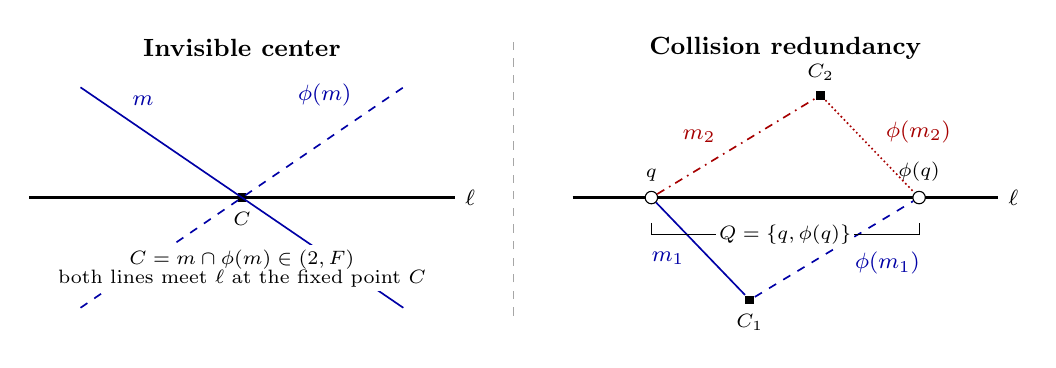
\begin{tikzpicture}[
  x=1cm,y=1cm,
  every node/.style={font=\footnotesize},
  carrier/.style={very thick},
  first/.style={semithick,blue!65!black},
  firstphi/.style={semithick,blue!65!black,dashed},
  second/.style={semithick,red!65!black,dash dot},
  secondphi/.style={semithick,red!65!black,densely dotted},
  fixed/.style={rectangle,fill=black,minimum size=3.2pt,inner sep=0pt},
  candidate/.style={circle,draw,fill=white,minimum size=4.5pt,inner sep=0pt}
]
  \begin{scope}
    \node[font=\small\bfseries] at (2.7,3.05) {Invisible center};
    \draw[carrier] (0,1.15) -- (5.4,1.15)
      node[right] {$\ell$};
    \node[fixed,label={[font=\scriptsize]below:$C$}] (c) at (2.7,1.15) {};
    \draw[first] (0.65,2.55) -- (4.75,-0.25)
      node[pos=0.13,above right] {$m$};
    \draw[firstphi] (0.65,-0.25) -- (4.75,2.55)
      node[pos=0.87,above left] {$\phi(m)$};
    \node[align=center,font=\scriptsize,fill=white,inner sep=1.5pt] at (2.7,0.25)
      {$C=m\cap\phi(m)\in\PG(2,F)$\\[-1pt]
       both lines meet $\ell$ at the fixed point $C$};
  \end{scope}

  \draw[dashed,black!35] (6.15,-0.35) -- (6.15,3.2);

  \begin{scope}[xshift=6.9cm]
    \node[font=\small\bfseries] at (2.7,3.05) {Collision redundancy};
    \draw[carrier] (0,1.15) -- (5.4,1.15)
      node[right] {$\ell$};
    \node[candidate,label={[font=\scriptsize]above:$q$}] (q) at (1.0,1.15) {};
    \node[candidate,label={[font=\scriptsize]above:$\phi(q)$}] (qp) at (4.4,1.15) {};

    \node[fixed,label={[font=\scriptsize]below:$C_1$}] (c1) at (2.25,-0.15) {};
    \node[fixed,label={[font=\scriptsize]above:$C_2$}] (c2) at (3.15,2.45) {};
    \draw[first] (q) -- (c1) node[pos=0.43,below left] {$m_1$};
    \draw[firstphi] (c1) -- (qp)
      node[pos=0.57,below right] {$\phi(m_1)$};
    \draw[second] (q) -- (c2) node[pos=0.43,above left] {$m_2$};
    \draw[secondphi] (c2) -- (qp)
      node[pos=0.57,above right] {$\phi(m_2)$};
    \draw[thin] (1.0,0.83) -- (1.0,0.68) -- (4.4,0.68) -- (4.4,0.83);
    \node[font=\scriptsize,fill=white,inner sep=1pt] at (2.7,0.68)
      {$Q=\{q,\phi(q)\}$};
  \end{scope}
\end{tikzpicture}
\caption{The two corrections to the first-order obstruction count on an
empty fixed carrier \(\ell\).  Left: when the fixed center
\(C=m\cap\phi(m)\) lies on \(\ell\), the conjugate secants meet the carrier
only at a fixed point and charge no candidate pair.  Right: two distinct
visible secant orbits have different fixed centers but charge the same
candidate \(Q=\{q,\phi(q)\}\); only one forbidden pair remains in the
support.  Solid/dashed and dash-dot/dotted lines distinguish the conjugate
secants in the two visible orbits.}
\label{fig:mate-line-correction}
\end{figure}


\begin{proposition}[Exact linewise correction]\label{prop:linewise}
For every empty fixed line $\ell$,
\begin{align}
 A_\ell&=M-B_\ell,\label{eq:visible-mass}\\
 |\cF_\ell|&=A_\ell-R_\ell,\label{eq:support}\\
 |\cQ_\ell\setminus\cF_\ell|+M
   &=N+B_\ell+R_\ell.\label{eq:linewise-balance}
\end{align}
Consequently the first-order identity
$|\cQ_\ell\setminus\cF_\ell|+M=N$ holds exactly when every secant orbit is
visible on $\ell$ and the visible charge map is injective.
\end{proposition}

\begin{proof}
Exactly $B_\ell$ of the $M$ secant orbits are invisible, proving
\eqref{eq:visible-mass}.  The support of the multiplicity function
$\mu_\ell$ is $\cF_\ell$, and for every positive integer $a$ one has
$1=a-(a-1)$.  Summing this equality over the support gives
\eqref{eq:support}.  Substitution into
$|\cQ_\ell\setminus\cF_\ell|=N-|\cF_\ell|$ gives
\eqref{eq:linewise-balance}.  Equality in the first-order identity is
equivalent to $B_\ell=R_\ell=0$.
\end{proof}

Let
\[
 L=\Npair(\cC),\qquad
 B=\sum_{\ell\in\cE}B_\ell,
 \qquad
 R=\sum_{\ell\in\cE}R_\ell.
\]

\begin{corollary}[Aggregate equality and excess]
\label{cor:aggregate}
The exact aggregate balance is
\begin{equation}\label{eq:aggregate}
  L+EM=EN+B+R.
\end{equation}
Thus $L+EM=EN$ if and only if every secant-orbit center avoids every empty
fixed carrier and every local visible charge is injective.  More generally,
for each integer $t\ge0$,
\[
  L+EM=EN+t\quad\Longleftrightarrow\quad B+R=t.
\]
\end{corollary}

This is an algebraic equality and excess classification.  It does not
classify the invariant arcs for which $L$ is small, and no such structural
inverse theorem is claimed.
